\documentclass[12pt,a4paper,twoside]{book}
\usepackage{graphicx}
\usepackage{setspace}	%double spacing for text, single for captions, footnotes, etc.
%\usepackage{hypernat} 	%substitut de cite que permet fer hyperlinks
\usepackage{natbib}		% substituye a 'hypernat' que funciona en Windows.
\usepackage[spanish]{babel}
\usepackage[utf8]{inputenc}
\usepackage{color}
\usepackage{hhline} 		% extended styles for tables
\usepackage{multirow}
\usepackage{subfigure}
\usepackage{acronym}
\usepackage{hyperref}
\usepackage{amsmath,amsmath,amssymb} 
\usepackage{fancyhdr}
\usepackage{epsfig, amsmath}
\usepackage{algorithm}
\usepackage{algorithmic}

% general settings
\hypersetup{
	linktocpage=true,
	colorlinks=true,
	linkcolor=blue,
	citecolor=blue,
}
\definecolor{Hgray}{gray}{0.6}

\newenvironment{definition}[1][Definition]{\begin{trivlist}
\item[\hskip \labelsep {\bfseries #1}]}{\end{trivlist}}

\setlength{\topmargin}{0cm}
\setlength{\textheight}{23cm}
\setlength{\textwidth}{17cm}
\setlength{\oddsidemargin}{0cm}
\setlength{\evensidemargin}{0cm}
\setlength{\headheight}{1cm}

% indica que las 'sub-sub-sections' sean numeradas y aparezcan en el indice
\setcounter{secnumdepth}{3}
\setcounter{tocdepth}{2}

% settings for code
\renewcommand{\algorithmicrequire}{\textbf{Entrada: }}
\renewcommand{\algorithmicensure}{\textbf{Salida: }}

%%%%%%%%%%%%
% DOCUMENT %
%%%%%%%%%%%%
\begin{document}

% portada
\newpage
\thispagestyle{empty}

\baselineskip 2em

%\vspace*{1cm}

\centerline{
\includegraphics[width=0.6\textwidth]{images/UOC-logo}}
\begin{center}
\textsc{Universitat Oberta de Catalunya (UOC) \\
 Máster Universitario en Ciencia de Datos (\textit{Data Science})\\}

%\centerline {\pic{UOC}{4cm}}

\vspace*{1.5cm}

\textsc{\Large TRABAJO FINAL DE MÁSTER}

\vspace*{0.5cm}

\textsc{\large Área: PLN}


%\textbf{\Huge VirtualTechLab Model: }

\vspace*{2.0cm}

\textbf{\Large Modelización de temas de llamadas en tiempo real}

\textbf{\large PEC II}

\vspace{2.5cm}
\baselineskip 1em

\baselineskip 2em
-----------------------------------------------------------------------------\\
Autor:      Manuel E. Gómez Montero\\
Tutora UOC:      Ana Valdivia Garcia\\
Tutor TE:      Antonio Fernández Gallardo\\
Profesor:   Jordi Casas\\
-----------------------------------------------------------------------------\\
\vspace*{1.5cm}
Madrid, \today

\end{center}

\newpage
\pagestyle{empty}
\hfill

\newpage
% abstract
\pagenumbering{roman} 
\setcounter{page}{1} 
\pagestyle{plain}

%%%%%%%%%%%%%%%%
%%% CREDITOS %%%
%%%%%%%%%%%%%%%%
%\chapter*{Créditos/Copyright}

%Una página con la especificación de créditos/copyright para el proyecto (ya sea aplicación por un lado y documentación por el otro, o unificadamente), así como la del uso de marcas, productos o servicios de terceros (incluidos códigos fuente). Si una persona diferente al autor colaboró en el proyecto, tiene que quedar explicitada su identidad y qué hizo.

%A continuación se ejemplifica el caso más habitual, aunque se puede modificar por cualquier otra alternativa:

%\vspace{1cm}

%\begin{figure}[ht]
%    \centering
%	
\includegraphics[scale=1]{images/license.png}
%\end{figure}

%Esta obra está sujeta a una licencia de Reconocimiento -  NoComercial - SinObraDerivada

%\href{https://creativecommons.org/licenses/by-nc-nd/3.0/es/}{3.0 España de CreativeCommons}.

%%%%%%%%%%%%%
%%% FICHA %%%
%%%%%%%%%%%%%
%\chapter*{FICHA DEL TRABAJO FINAL}

%\begin{table}[ht]
%	\centering{}
%	\renewcommand{\arraystretch}{2}
%	\begin{tabular}{r | l}
%		\hline
%		Título del trabajo: & Descriptivo del trabajo\\
%		\hline
%       Nombre del autor: & Nombre y dos apellidos\\
%		\hline
%        Nombre del colaborador/a docente: & Nombre y dos apellidos\\
%		\hline
%        Nombre del PRA: & Nombre y dos apellidos\\
%		\hline
%        Fecha de entrega (mm/aaaa): & MM/AAAA\\
%		\hline
%        Titulación o programa: & Plan de estudios\\
%		\hline
%        Área del Trabajo Final: & El nombre de la asignatura de TF\\
%		\hline
%        Idioma del trabajo: & Catalán, español o inglés\\
%		\hline
%        Palabras clave & Máximo 3 palabras clave\\
%		\hline
%	\end{tabular}
%\end{table}

%%%%%%%%%%%%%%%%%%%
%%% DEDICATORIA %%%
%%%%%%%%%%%%%%%%%%%
%\chapter*{Dedicatoria/Cita}

%Breves palabras de dedicatoria y/o una cita.

%%%%%%%%%%%%%%%%%%%
%%% Agradecimientos %%%
%%%%%%%%%%%%%%%%%%%
%\chapter*{Agradecimientos}



%%%%%%%%%%%%%%%%
%%% RESUMEN  %%%
%%%%%%%%%%%%%%%%
\chapter*{Resumen}
\addcontentsline{toc}{chapter}{Abstract}


Un call-center es el área de una empresa el cuál se encarga de recibir y transmitir llamadas desde o hacia clientes, socios comerciales u otras compañías externas. Debido a la gran cantidad de información que se transfiere en estos centros, resulta una tarea esencial optimizar el tiempo de respuesta para así reaccionar en tiempo real a las peticiones de los clientes y mejorar la percepción que estos tienen sobre la compañía. 

Una manera de mejorar el rendimiento es detectar el tema de las llamadas  mediante técnicas de \textit{machine learning} dando la posibilidad a la empresa de reaccionar en tiempo real, en función de la temática que se este tratando en cada momento. 



%El documento que se presenta tiene como objetivo final mejorar la operatividad del \textit{call-center}  de una gran empresa, extrayendo mediante técnicas de \textit{machine learning} la temática de las llamadas que se realizan al mismo y dando la posibilidad a la empresa de reaccionar en tiempo real, en función de la temática que se este tratando en cada momento. 

El sistema que se presenta en el documento nos permite, a partir de la transcripción de las llamadas al \textit{call-center} de Telefónica España, descubrir en tiempo real la temática de las mismas. Esta modelización de \textit{topics} se ha realizado utilizando métodos de Procesamiento de Lenguaje Natural y aprendizaje profundo. El sistema realiza la clasificación de las nuevas llamadas en tiempo real, permitiendo a los usuarios visualizar la evolución en la temática de las mismas y generar alertas en base a anomalías.  


%TODO Es un borrador volver al  resumen una vez acabado el proyecto.
\onehalfspacing

\vspace{1.5cm}

\textbf{Palabras clave}: ``natural language processing'', ``sentiment analysis'', ``real time'', ``call center'', ``topic modeling'', ``deep learning''
\newpage

\pagestyle{fancy}
\renewcommand{\chaptermark}[1]{ \markboth{#1}{}}
\renewcommand{\sectionmark}[1]{\markright{ \thesection.\ #1}}
\lhead[\fancyplain{}{\bfseries\thepage}]{\fancyplain{}{\bfseries\rightmark}}
\rhead[\fancyplain{}{\bfseries\leftmark}]{\fancyplain{}{\bfseries\thepage}}
\cfoot{}

% indice
\cleardoublepage
\phantomsection
\addcontentsline{toc}{chapter}{Índice}
\tableofcontents
% listado de figuras
\cleardoublepage
\phantomsection
\addcontentsline{toc}{chapter}{Llistado de Figuras}
\listoffigures
% listado de tablas
\cleardoublepage
\phantomsection
\addcontentsline{toc}{chapter}{Listado de Tablas}
\listoftables

\thispagestyle{empty}

\pagenumbering{arabic}

\pagestyle{fancy}
\renewcommand{\chaptermark}[1]{ \markboth{#1}{}}
\renewcommand{\sectionmark}[1]{\markright{ \thesection.\ #1}}
\lhead[\fancyplain{}{\bfseries\thepage}]{\fancyplain{}{\bfseries\rightmark}}
\rhead[\fancyplain{}{\bfseries\leftmark}]{\fancyplain{}{\bfseries\thepage}}
\cfoot{}

\onehalfspacing

% capitulos del documento
\chapter{Introducción}
\label{chapter:introduccion}

Este primer capítulo del trabajo tiene como objetivo presentar, a grandes rasgos, la propuesta (sección \ref{section:intro:descripcion}), los objetivos que pretendemos lograr (sección \ref{section:intro:objetivos}), la motivación que nos ha llevado a abordar este proyecto (sección \ref{section:intro:motivacion}) y un repaso a las tareas que serán necesarias para la ejecución del mismo (sección \ref{section:intro:planificacion}). 


\section{Descripción general de la propuesta}
\label{section:intro:descripcion}
En los últimos años, la explosión ingente en la generación de datos y el avance en las capacidades tecnológicas que nos permiten recolectar, almacenar y procesar los datos generados; han provocado que empecemos a abordar el estudio de otro tipo de datos no estructurados que antes no se podían analizar como imágenes, textos, audios, etc. Como resultado, diferentes áreas del conocimiento (Procesamiento del Lenguaje Natural, Análisis de Imágenes) han experimentado un creciente interés tanto en la comunidad científica como en el mundo de los negocios. 


Dentro de los datos no estructurados, una de las fuentes de información con mayor potencial en todas las grandes empresas que prestan servicio al público general, son las llamadas que los clientes realizan a su \textit{call-center}, ya que nos permiten obtener una idea de la percepción que los clientes tienen de nuestra empresa y de sus preocupaciones en cada momento. 

La propuesta que pretendemos abordar en este trabajo consiste en extraer la temática de  estas llamadas en el momento en el que son capturadas. Aunque actualmente esta captura se hace periódicamente pretendemos construir una solución que nos permita el tratamiento de las mismas en tiempo real o streaming, y de esta manera mejorar el rendimiento de estos centros. %para que esta solución sea válida en un futuro próximo cuando se aumente la frecuencia de ingesta. 

Esta extracción en tiempo real nos permitirá conocer cómo evolucionan los temas que tratan nuestros clientes cuando llaman a nuestro \textit{call-center} para así poder reaccionar inmediatamente ante una preocupación concreta. 


\section{Motivación}
\label{section:intro:motivacion}
La motivación que nos ha llevado a acometer un proyecto de esta naturaleza viene originada por diferentes factores que están ligados tanto al negocio como a las capacidades técnicas disponibles en la empresa. 

Por un lado, la capacidad de obtener la temática de las llamadas en tiempo real se presenta como una oportunidad de mejorar la operatividad de un \textit{call-center} y por ende la satisfacción de los clientes, permitiéndonos entenderlos mejor y así reaccionar de una manera ágil a sus necesidades reales.

Desde el punto de vista técnico, también es el momento ideal para emprender este proyecto debido tanto a la disponibilidad periódica de transcripciones de las llamadas, que nos permiten ahorrarnos el paso de realizar un \textit{Speech 2 Text} para obtener nuestro conjunto de datos; como al aumento de capacidades técnicas en la empresa que nos permitirán tanto entrenar nuestros modelos, como poder tratar y explotar los datos en tiempo real. 


\section{Objetivos}
\label{section:intro:objetivos}
En este apartado definiremos los objetivos que se pretenden conseguir con este proyecto. Estos objetivos deben ser \textit{SMART}, es decir: 

\begin{itemize}
	\item \textit{\textbf{S}pecific}: Deben plantearse de una forma detallada y concreta.
	\item \textit{\textbf{M}easurable}: Deben poder medirse con facilidad.
	\item \textit{\textbf{A}chievable}: Deben ser objetivos realistas.
	\item \textit{\textbf{R}elevant}: Tienen que ser relevantes para la empresa y ofrecernos un beneficio claro.
	\item  \textit{\textbf{T}imely}: Estos objetivos tienen que tener un tiempo establecido.
\end{itemize}




El objetivo general es optimizar el proceso de atención de llamadas en el call-center mediante técnicas de Procesamiento del Lenguaje Natural y Aprendizaje Profundo. Concretamente, los objetivos específicos que se pretenden conseguir con este proyecto son: 

\begin{itemize}
	\item \textbf{Construir un modelo que nos permita extraer la temática de las llamadas} a partir de su transcripción a texto. Este objetivo debemos alcanzarlo en la fase de modelado y podremos medir su éxito atendiendo al porcentaje de llamadas que podamos clasificar correctamente en un proceso de test. Se trata del objetivo principal del proyecto.
	\item Desarrollar un mecanismo que nos permita \textbf{extraer esta temática para nuevas llamadas en tiempo real}. De este modo tendremos un sistema vigente cuando la frecuencia en la recepción de las llamadas aumente. Este objetivo se deberá alcanzar en la fase de productivización. 
	\item Disponer de una\textbf{ visualización en tiempo cuasi real} para que pueda visualizarse la evolución de las temáticas a lo largo del tiempo. Este objetivo se deberá alcanzar en la fase de productivización. 
	\item Proporcionar un \textbf{sistema de alertado} que nos permita detectar anomalías en el número de llamadas que se reciben de un determinado tema. Este objetivo se deberá alcanzar en la fase de productivización.
\end{itemize}

En las conclusiones de este proyecto se evaluará el éxito o fracaso del mismo en función del grado de cumplimiento de estos objetivos.

\section{Tareas y planificación}
\label{section:intro:planificacion}
El proyecto se llevará a cabo desde el 16 de Septiembre hasta el 20 de Febrero. Para poder abordar la ejecución del  mismo se han extraído las siguientes tareas principales: 


\begin{figure}[!ht]
	\centering
	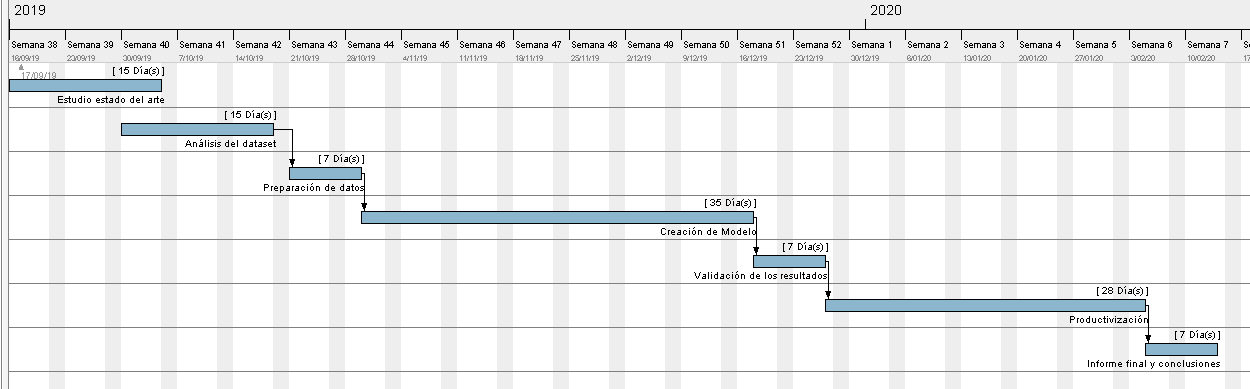
\includegraphics[width=\textwidth]{images/intro/gantt}
	\caption{Diagrama de Gantt}
	\label{fig:gantt}
\end{figure}


\begin{itemize}
	\item \textbf{Estudio estado del arte}: En esta fase se realizará una prospección para conocer el estado del arte en todos los puntos relacionados con el proyecto: Procesamiento del Lenguaje Natural, tecnologías de tratamiento de datos en tiempo real y \textit{Big Data}. 
	
	\item \textbf{Análisis del \textit{dataset}}: El propósito de esta tarea es entender el \textit{dataset}  y estudiar las posibilidades del mismo. 
	
	\item\textbf{ Preparación del \textit{dataset}}: Una vez realizado el estudio del \textit{dataset} es necesario realizar labores de limpieza y transformación de los datos de modo que estos datos sean válidos para nuestro objetivo.
	
	\item \textbf{Creación del modelo}: En esta fase se procederá a la creación de un modelo capaz de obtener los temas de los que habla una determinada llamada. Este modelo será el \textit{core} de nuestro proyecto.
	
	\item \textbf{Validación de los resultados}: Una vez entrenado el modelo será necesario validar los resultados obtenidos para poder evaluar la bondad de nuestro modelo. 
	
	\item\textbf{ Productivización}: El trabajo no acaba con la creación de un buen modelo que nos permita extraer los temas de nuestras llamadas. Este modelo tendrá que ser puesto en producción y permitir al usuario final extraer los temas de las llamadas en tiempo real y darle la opción de crear alarmas basadas en la variación del número de eventos (llamadas) de un determinado tema.
	\item\textbf{ Informe final y conclusiones}: Por último, una vez llevado a a producción nuestro modelo, se realizará un informe final donde, entre otros puntos, se evaluarán los resultados obtenidos y se extraerán conclusiones y pasos futuros.
\end{itemize} 

\begin{figure}[!ht]
	\centering
	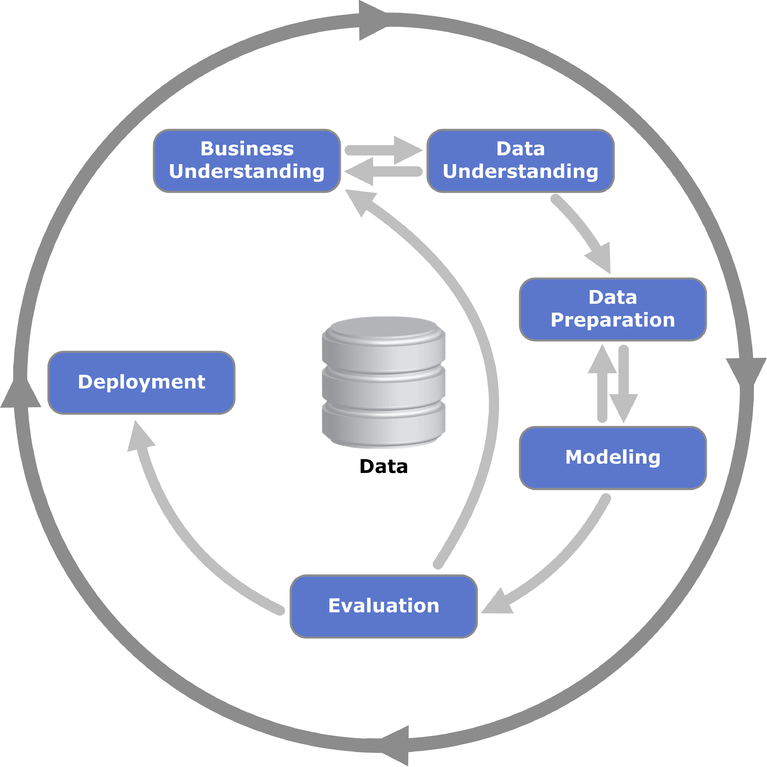
\includegraphics[width=0.63\textwidth]{images/intro/crispdm}
	\caption{Fases del modelo CRISP-DM}
	\label{fig:crispdm}
\end{figure}


Estas fases están basadas en el estándar \textbf{\textit{CRISP-DM}} (\cite{crispdm}), añadiendo una última tarea para nuestro informe final, \textit{CRISP-DM} nos proporciona una descripción del ciclo de vida de los proyectos de minería de datos de un modo bastante similar al que se aplica en los modelos de ciclo de vida de desarrollo \textit{software}.


 

En la Figura \ref{fig:crispdm} se observa el diseño de este modelo y cómo representa el ciclo de vida de un proyecto de minería de datos. En la imagen podemos ver en primer lugar un círculo exterior que refleja la naturaleza cíclica de los proyectos de minería de datos, además vemos cómo la secuencia de tareas no es rígida, pudiendo saltar hacia adelante o atrás entre tareas. En la gráfica se representan mediante flechas las dependencias más importantes y usuales entre tareas.

En nuestro desarrollo usaremos este modelo, aunque en el diagrama de la Figura \ref{fig:gantt} aparezca una secuencia de tareas más rígida, será usual, por ejemplo, el salto recíproco entre las fases de preparación de los datos y creación del modelo.




% bibliografia
\addcontentsline{toc}{chapter}{Bibliografía}
\bibliographystyle{plain}
\bibliography{referencias}

\end{document}